% 環境設定
% !TEX program = xelatex
% !TEX encoding = UTF-8
% !BIB program = biber
\documentclass[12pt,a4paper]{article}

% 字體套件
\usepackage{fontspec}
\usepackage[BoldFont]{xeCJK}
% 字體設定
\setCJKmainfont{DFKai-SB}     % 標楷體
\setmainfont{Times New Roman}
% 中文自動換行
\XeTeXlinebreaklocale "zh"             
\XeTeXlinebreakskip = 0pt plus 1pt     

% 紙張格式
\usepackage{geometry}
\geometry{
 a4paper,
 left=12.7mm,
 right=12.7mm,
 top=12.7mm,
 bottom=12.7mm,
}

% 套件
\usepackage{amssymb}
\usepackage{mathtools}
\usepackage{microtype}
\usepackage{enumitem}
\usepackage{dirtytalk}
\usepackage[figurename=圖]{caption}
\usepackage{float}
\usepackage{subcaption}
\usepackage{fancyhdr}
\usepackage{graphicx}
\usepackage{hyperref}
\usepackage{lastpage}
\usepackage{cite}

% 設定
\renewcommand{\tablename}{表}
\pagestyle{fancy}
\fancyhead{}
\fancyfoot{}
\renewcommand{\headrulewidth}{0pt}
\renewcommand{\footrulewidth}{0pt}
\setlength{\headwidth}{\textwidth}

% \lfoot{表 CM03}
\rfoot{共~~\pageref{LastPage}~~頁~~第{~~\thepage~~}頁}

\begin{document}

\noindent{\bf \large 基於機器學習實現智慧化水質分析與評估系統} 

\begin{enumerate}
\item[(一)] 研究計畫之背景。
\begin{enumerate}[label=\arabic*.]
\item 研究計畫之背景\\
  本研究旨在開發並實現具機器學習(Machine Learning, ML)功能的智慧化水質分析與評估系統,以解決目前水質資料分析缺乏高效率方法的問題。研究作者曾擔任科技部計畫兼任研究助理,協助執行「運用智慧型綠能永續景觀噴泉促進環境保育效益之研究」(計畫編號:MOST 110-2410-H025-024),該計畫運用物聯網(Internet of Things, IoT)技術蒐集南投麒麟潭的水質資料。藉由該計畫經驗發現自動化運行的結果相較於人工記錄更有效率,但後續資料分析仍需耗費大量工作時間。
\item 研究問題\\
  在水質資料分析方面,除了使用Microsoft Excel直接計算外,通常會使用如Statistical Analysis System(SAS)或Statistical Product and Service Solutions(SPSS)等統計專有軟體(Proprietary Software)。然而,這些軟體為專有(Proprietary)且非開源,不僅需要額外購買授權,還需投入時間學習才能熟練使用。由於其操作高度依賴使用者的專業知識,分析結果可能因個人經驗而有所差異。由於這些軟體無法修改與物聯網設備直接進行資料串聯傳輸,造成未來計畫整合實現自動化資料收集與資料分析的障礙。
\item 研究原創性\\
  近十年來,人工智慧(Artificial Intelligence, AI)從理論發展到實際應用,各種AI等工具也被廣泛運用於日常問題成為解決方案\cite{ref1}。本研究運用人工智慧中的機器學習技術,開發一套智慧化水質分析與評估系統,實現更高效且易於操作的創新水質分析方法。不同於傳統統計軟體需要人工輸入與分析,本系統將結合自動化資料處理與機器學習演算法,以提升水質分析的準確性與效率。此外,本研究將探索AI在水資源管理與環境保育領域的創新應用,提供創新的智慧化水質資料分析方案。\\  
  為了找出最適合水質分析的機器學習模型,本研究針對XGBoost、LightGBM、支援向量機(Support Vector Machine, SVM)、隨機森林(Random Forest, RF)、多元多項式迴歸(Multiple Polynomial Regression, MPR)以及線性迴歸(Linear Regression, LR)等多種模型進行比較與評估。透過實驗分析與比較不同模型在水質資料分析準確度、計算效能與資料適應性的表現,進一步應用於改良水質分析,使系統能夠有效應對水體環境的分析與評估需求。\\
  實驗設計包括使用先前於「運用智慧型綠能永續景觀噴泉促進環境保育效益之研究」計畫中,使用物聯網設備實際蒐集的水質資料,加上環境部環境資料開放平臺公開資料使用,特徵選擇包括溶解氧(DO)、生化需氧量(BOD)、氨氮(NH3-N)、電導度(EC)和懸浮固體(SS)等關鍵指標。在訓練過程中,使用水體品質指標(Water Quality Index, WQI$_5$)作為標記資料進行監督式學習。
    % 圖 1
    \begin{figure}[H]
        \centering
        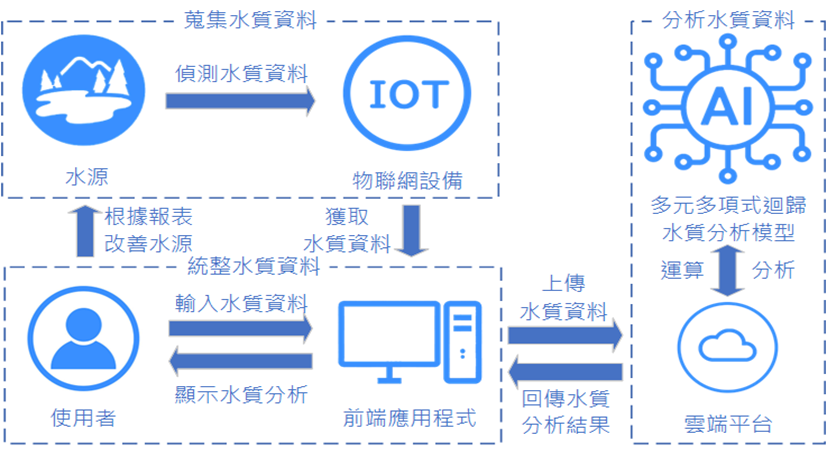
\includegraphics[width=0.75\textwidth]{resources/image/使用情境圖.png}
        \caption{使用情境圖}
        \label{fig:usage_scenario}
    \end{figure}
\item 研究重要性\\
  在過去十年內,人工智慧的研究從長期被忽視的陰霾中走了出來,被人們看見了希望且掀起了新一波風潮\cite{ref2},而水資源管理與環境生態保育是全球關注的議題,而水質分析與評估是確保水資源安全的重要環節。本研究透過機器學習技術,克服傳統方法的效率瓶頸,降低對專業知識依賴,使水質資料分析變得更有效且易於操作,提升水質資料分析技術的普及性與可行性。\\  
  本研究針對XGBoost、LightGBM、支援向量機(SVM)、隨機森林(RF)、多元多項式迴歸(MPR)以及線性迴歸(LR)等機器學習模型進行獨立訓練,並透過決定係數($R^2$)、均方根誤差(Root Mean Square Error, RMSE)、平均絕對誤差(Mean Absolute Error, MAE)以及殘差分析等指標評估各模型在水質資料分析上的準確性。\\  
  透過實驗分析,我們發現[TODO]。這些結果有助於選擇最適合水質資料分析的機器學習模型,進一步提升水資源管理的準確度,為環境監測技術與未來相關研究的發展提供有效的參考依據。
\item 預期影響性\\
  本研究的智慧化水質分析與評估系統結合了模型比較實驗與系統開發,有望在以下方面產生影響:
    \begin{enumerate}[label=1-5-\arabic*.]
        \item 技術創新:人工智慧未來將成為人類不可或缺的夥伴\cite{ref3},本研究在水質資料分析引入機器學習技術,提升分析準確性與自動化程度。
        \item 環境保育:能夠在水資源管理方面準確且有效地發現水質變化,改善水體生態環境。
        \item 跨領域應用:本研究結合了資訊工程、人工智慧、水資源管理和環境生態保育等不同領域,未來也可擴展應用於不同環境監測領域,例如空氣品質監測或污染物分析,促進人工智慧在環境科學中的應用。
    \end{enumerate}
\item 國內外研究情況\\
  本研究作者先前參與的計畫已經使用物聯網技術進行水質資料的採集,這種方法在環境監測中已經相當普遍。然而,目前國內外針對水質資料分析的智慧化系統,特別是結合機器學習技術的水質分析系統相對較少。機器學習技術在水質評估中的應用已被證明是有效的,並逐漸成為水資源管理的重要分析工具\cite{ref4},應用各種技術構建學習模型,能夠達成提供即時準確水質資訊的目的,期望得以透過早期診斷水質異常以改善公共健康\cite{ref5}因此,本研究具有創新性和獨特性,有助於填補水質資料分析中高效方法的空白。
\item 重要參考文獻\\
  隨著人工智慧發展,各種機器學習模型也如雨後春筍般出現。模型實作上如開發一種基於多元多項式迴歸(MPR)的機器學習模型,在該研究中以模型與線性迴歸及支援向量機模型進行比較,發現MPR在性能評估指標包含R²(R-squared)和RMSE(Root-Mean-Square Error)上皆優於另外兩個模型\cite{ref6},其提出的MPR公式如(1)所示,其中 $\hat{y}$ 是輸出變數,$w_0$ 是截距,$w_1, w_2, \ldots, w_s$ 為多項式迴歸係數,$x$ 為輸入變數,表示具有 $n$ 個輸入變數和階數($s > 1$)的 MPR 系統。加上其他研究成果使用MPR模型驗證其預測結果\cite{ref7},如圖2所示,MPR建立了一個六元多項式迴歸模型,結果顯示其訓練集的MAPE(Mean Absolute Percentage Error)為1.873\%,MAE(Mean Absolute Error)為(TODO待確認),證明了MPR模型在水質資料分析上的優越性\cite{ref8}。這些研究成果將有助於本研究的模型選擇與效能評估,也因此本研究前期採用MPR模型作為基準模型進行比較。\\
    \begin{equation}
        \hat{y} = w_0 + \sum_{i_1=1}^{n} w_{i_1} x_{i_1} + \sum_{i_1=1}^{n} \sum_{i_2=i_1}^{n} w_{i_1 i_2} x_{i_1} x_{i_2} + ... \\
        + \sum_{i_1=1}^{n} \sum_{i_2=i_1}^{n} ... \sum_{i_k=i_{k-1}}^{n} w_{i_1 i_2 ... i_k} x_{i_1} x_{i_2} ... x_{i_k}
    \end{equation}
  另外,隨著近年來XGBoost與LightGBM等新興模型在機器學習領域中的崛起,本研究在中後期將其納入比較範疇,XGBoost在資料科學領域中被廣泛使用,也在Kaggle許多機器學習及競賽中取得最佳結果,其特點為有非常強的擴展性(Scalibility)與性能,可以使用相對其他模型更少的系統資源,擴充數十億級別的資料\cite{ref9}。而LightGBM是一種高效能的梯度提升決策樹,在傳統Gradient Boosting Decision Tree(GBDT)演算法上加入使用Gradient-based One-Side Sampling(GOSS)和Exclusive Feature Bunding (EFB),並顯示出LightGBM相較傳統的GBDT加快了20倍以上的速度,同時也並未降低準確性\cite{ref10}。\\
  綜合以上重要參考文獻,本研究對XGBoost、LightGBM、支援向量機(Support Vector Machine, SVM)、隨機森林(Random Forest, RF)、多元多項式迴歸(Multiple Polynomial Regression, MPR)以及線性迴歸(Linear Regression, LR)等多種模型進行比較與評估,期望找出最適合水質分析的機器學習模型,並提升水質分析的準確性與效率。
    % 圖 2
    \begin{figure}[H]
        \centering
        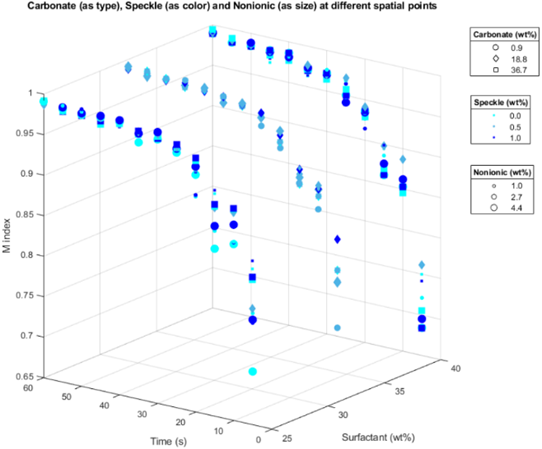
\includegraphics[width=0.5\textwidth]{resources/image/Canamero et al.(2023).png}
        \caption{Canamero等人提出的六元MPR模型}
        \label{fig:MPR_validation}
    \end{figure}
\end{enumerate}

\item[(二)] 研究方法、進行步驟及執行進度。
\begin{enumerate}[label=\arabic*.]
\item 研究方法\\
  本研究開發之智慧化水質分析與評估系統採用前後端分離架構,透過應用程式介面(Application Programming Interface, API)進行資料傳遞與呼叫。後端(Back-end)水質資料分析模型以Python程式語言開發,運用NumPy、Pandas及Scikit-learn等工具進行水質資料的處理和分析。前端(Front-end)則以JavaScript語言的React Native框架開發行動裝置應用程式,實現跨系統平臺操作。此架構的水質資料分析模型開發可歸納為四個步驟:匯入資料、資料處理、特徵工程及模型訓練與評估。系統建置完成後,使用者在前端行動裝置應用程式中只需輸入欲分析的水質資料,即可經由已訓練完成的機器學習模型進行分析,再於使用者介面(UI)將產生一份分析報表,包括水質狀況的綜合評分以及狀態說明。\\
    \begin{figure}[H]
        \centering
        \begin{minipage}[t]{0.4\textwidth}
            \centering
            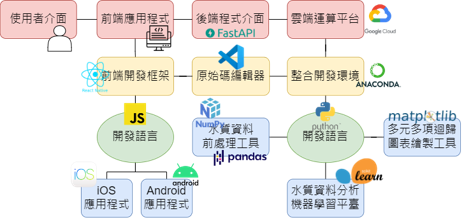
\includegraphics[width=\textwidth]{resources/image/開發架構圖.png}
            \caption{系統程式開發架構圖}
            \label{fig:development_architecture}
        \end{minipage}
        \hspace{0.01\textwidth}
        \begin{minipage}[t]{0.4\textwidth}
            \centering
            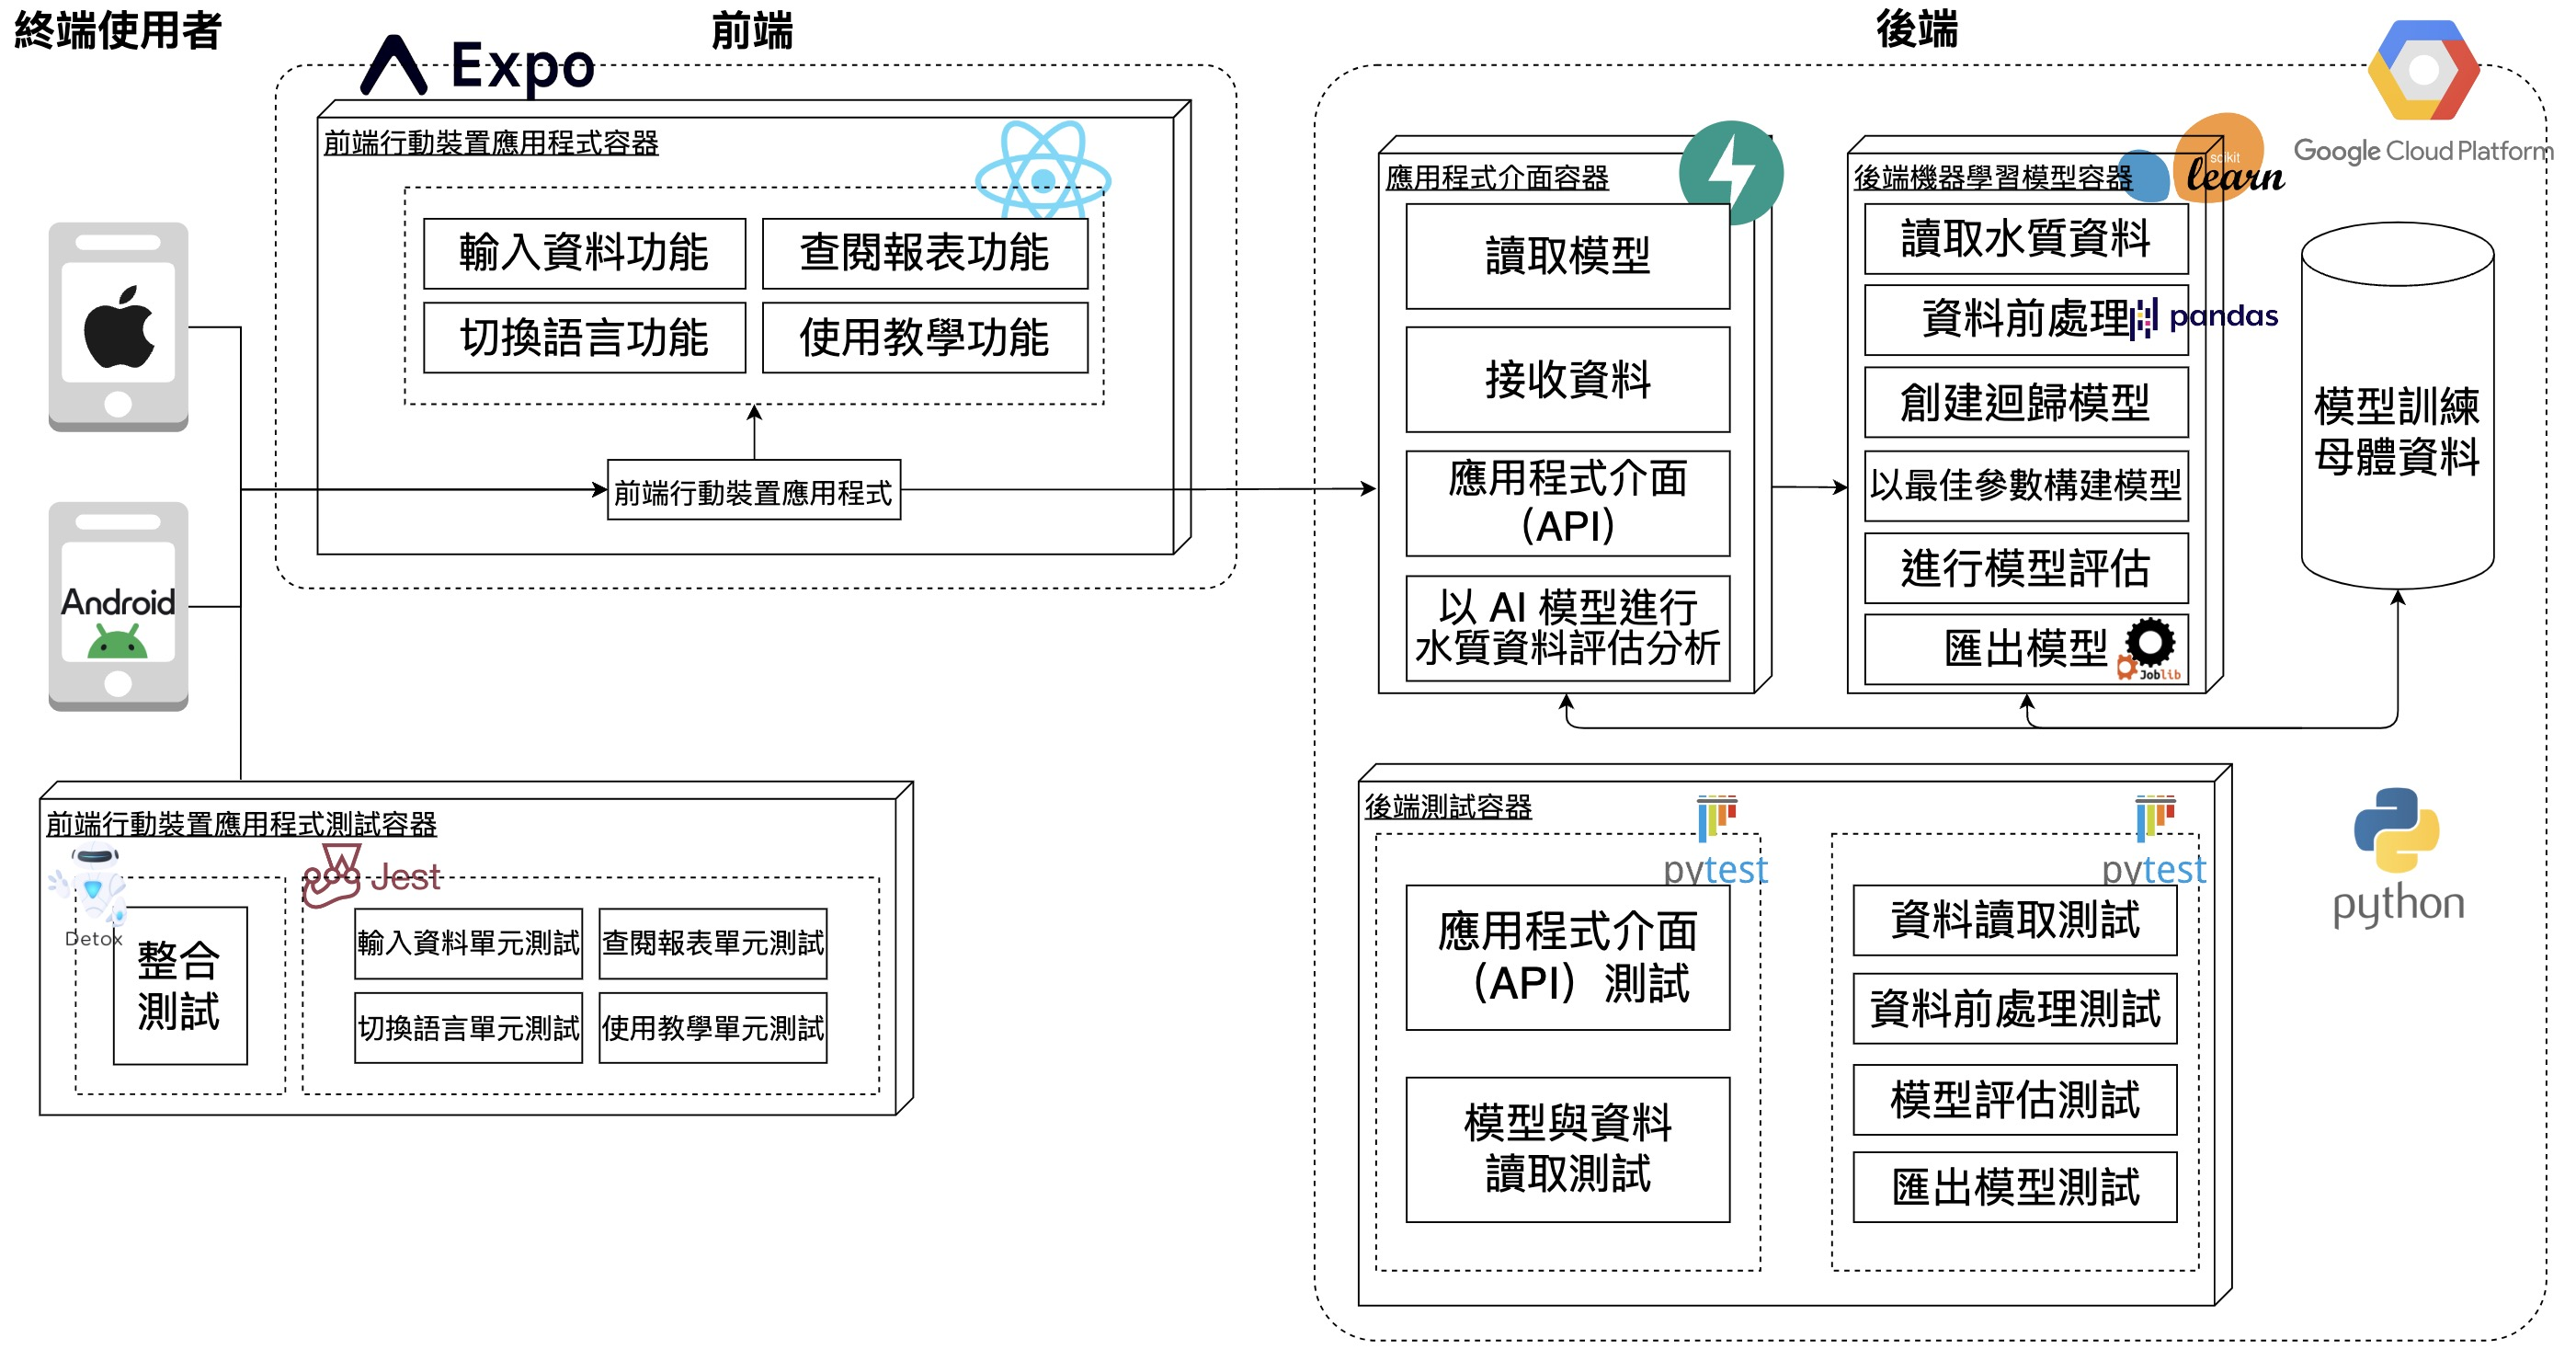
\includegraphics[width=\textwidth]{resources/image/部署圖.jpg}
            \caption{系統部署圖}
            \label{fig:deployment_diagram}
        \end{minipage}
    \end{figure}
  在模型開發過程中,我們認為機器學習技術不僅適用於水質資料分析,也能拓展到其他相關領域。除了前期使用的MPR模型外,我們還加入XGBoost和LightGBM等新興優秀模型進行比較,以尋找最適合解決問題的方案。研究工具方面涵蓋了機器學習程式語言(2-1-1)、開發環境(2-1-2)、功能函式庫(2-1-3)及前端開發工具(2-1-4),用以構建一套完整的水質資料分析與評估系統,並確保能挑選出最佳模型。各項工具分述如下:
    \begin{enumerate}[label=2-1-\arabic*.]
        \item 機器學習語言\\
          近年來Python在人工智慧領域中具有顯著影響力,因其優秀的資料處理與分析能力,支援各式開源函式庫使得Python成為資料分析的熱門選擇\cite{ref12},且能夠有效處理即時、大型和非結構化資料\cite{ref13},對於本研究進行各式水質資料分析的研究具有明顯的優勢。
        \item 機器學習環境\\
          本研究機器學習環境主要分為(A)雲端運算平臺及(B)開發環境。正如所言「工欲善其事,必先利其器」,為了能夠有效率地進行整體系統的各項開發,並在完成後部署於雲端運算平臺。 
                    \begin{enumerate}[label=\Alph*.]
                        \item 雲端運算平臺\\
                          本研究運用機器學習框架-Scikit-learn進行功能開發,Scikit-learn著重高效能的運算資源利用,符合智慧化水質資料分析的應用需求。此外,亦將建置雲端平臺-開發與部署所建置之MPR模型於Google Cloud Platform(GCP),GCP為一種基礎結構即服務(IaaS)平臺,提供於雲端部署機器模型之能力。 
                        \item 開發環境\\
                          本研究採用Visual Studio Code作為整合開發環境(Integrated Development Environment, IDE),並透過Docker實現容器化開發。可以直接將所開發之機器學習模型與應用程式部署至雲端平臺,運用分散式架構使得本研究具備處理和運算大量水質資料的能力。
                    \end{enumerate}
        \item 功能函式庫\\
          程式開發所需之功能函式庫分為:(A)資料處理工具、(B)機器學習框架、(C)圖表繪製工具及(D)應用程式介面。實作上以模組化方式結合各項工具能有助於完成水質分析模型的建構,相關說明如下:
            \begin{enumerate}[label=\Alph*.]
                \item 資料處理工具\\
                  本研究以NumPy及Pandas作為資料處理工具,NumPy是Python程式語言中支援科學和數值計算的函式庫,也相容於Pandas、Matplotlib和Scikit-learn等工具\cite{ref14}。NumPy作為資料處理的主要工具是因為它提供了科學計算所需的基本資料結構\cite{ref15}。同時NumPy也提供豐富的數學運算、資料讀寫、線性代數、傅立葉變換和隨機數生成等功能函式\cite{ref16}。使用NumPy得以更有效率地處理原始資料,進一步提升程式的開發效率。而Pandas建立於NumPy的基礎之上,是一種用於格式化資料分析的開源Python函式庫,它能夠處理類似電子試算表格式的輸入資料,可以快速地進行資料載入、操作、對齊和合併等功能\cite{ref17}。
                \item 機器學習框架\\
                  本研究採用了Scikit-learn作為機器學習框架,以建構研究所需的各種機器學習模型模型\cite{ref18}。支援Python程式的機器學習框架之中,Scikit-learn提供多樣的演算法,其特色包括具有良好的應用程式介面(Application Programming Interface, API)、詳細文檔說明及技術支援\cite{ref19}。由於Scikit-learn具有輕量而高效的特性,可使本研究實作能夠有效率地達到智慧化水質資料分析的應用需求。
                \item 圖表繪製工具\\
                  Matplotlib是一個多功能的Python繪圖函式庫,具有產生各種類型和格式圖表的功能,包括折線圖、散布圖、熱圖、直方圖、圓餅圖和立體圖形,同時也支援動畫和互動顯示\cite{ref20}。運用Matplotlib能夠以視覺化方式呈現多元多項式迴歸運算後的水質資料分析結果,使模型訓練結果呈現更生動以提升可讀性。
                \item 應用程式介面\\
                  本研究以FastAPI作為應用程式界面(API)框架,FastAPI是一個新興但可靠的API框架\cite{ref21},能夠快速且有效地於Python建立RESTful API伺服器。機器學習模型與使用FastAPI服務的前端整合,能夠相較使用如Flask等其他API框架的效能提高了45\%\cite{ref22}。使用FastAPI建立API,有助於前後端之間的通訊與資料傳遞,實現智慧化水質分析與評估系統的系統化架構。
            \end{enumerate}
        \item 前端開發工具\\
          在進行前端應用程式開發的過程中,本研究採用React Native框架。此框架由Meta公司基於React框架與JavaScript語言設計開發,重點在於能夠開發跨操作系統運行的行動裝置應用程式,作業系統支援包括Android及iOS\cite{ref23}。使用React Native不僅能夠直接進行跨系統平臺開發,還能顯著提升行動裝置應用程式開發的速度。使得本研究在開發具機器學習功能之智慧化水質分析與評估系統時,前端開發的效率明顯優於單獨針對Android或iOS進行開發的方法。
    \end{enumerate}
\item 研究步驟\\
  本研究所設計之多元多項式迴歸模型開發與實驗步驟流程如圖所示,可分為(2-2-1)資料取得、(2-2-2)資料前處理、(2-2-3)模型選擇與比較、(2-2-4)超參數調整、(2-2-5)改良與測試及(2-2-6)實現系統化,整體系統化作業流程包含起始於資料取得、模型完成與最終實際應用於水質分析,以實現「基於機器學習實現智慧化水質分析與評估系統」為目標。
    \begin{figure}[H]
        \centering
        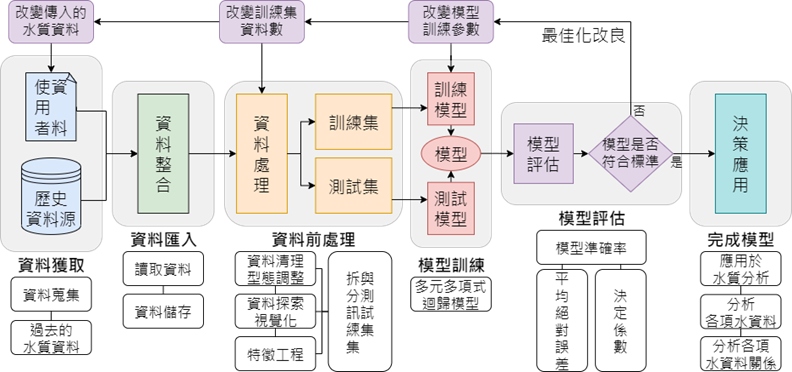
\includegraphics[width=0.8\textwidth]{resources/image/模型建構流程圖.png}
        \caption{模型建構流程圖}
        \label{fig:research_steps}
    \end{figure}
    \begin{enumerate}[label=2-2-\arabic*.]
        \item 資料取得\\
          本研究將參考「運用智慧型綠能永續景觀噴泉促進環境保育效益之研究」計畫(編號:MOST110-2410-H025-024)所蒐集的水質資料,並結合中華民國環境部全國環境水質監測資訊網的公開資料,共計蒐集了87,005筆水質資料。本研究所採用的水質參數包括溶氧量(DO)、生物需氧量(BOD)、懸浮固體(SS)、氨氮(NH3-N)及導電度(EC)。研究中將使用多元多項式迴歸(MPR)模型對各項水質資料進行機器學習分析。如圖所示,不同資料之間存在交互影響水質健康的關係,例如:DO濃度越高,NH3-N及EC濃度越低;NH3-N濃度越高,EC越高。此外,DO與水質綜合評分之關係顯示其為重要指標之一,而BOD、NH3-N、EC及SS與水質綜合評分之關係則顯示其為水質污染的指標。        
            \begin{figure}[H]
                \centering
                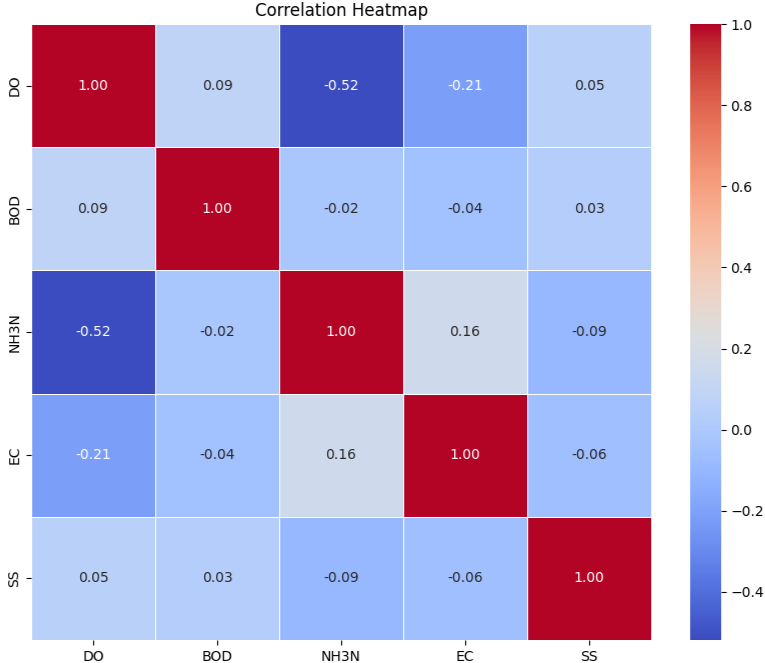
\includegraphics[width=0.5\textwidth]{resources/image/heatmap.png}
                \caption{相關性分析矩陣}
                \label{fig:correlation_matrix}
            \end{figure}
        \item 資料前處理\\
          在進行機器學習模型訓練前,需對蒐集的原始資料進行前處理,以減少母體資料中的不確定性。此過程可以透過Pandas來完成,主要步驟包括:(A)遺失值處理、(B)異常值處理、(C)標準化、(D)資料拆分及(E)特徵工程等。各項操作重點說明如下:
            \begin{enumerate}[label=\Alph*.]
                \item 遺失值處理\\
                  在機器學習資料前處理階段,需要處理原始水質資料中的遺失值(Missing Value),處理方式通常有兩種:直接刪除或進行填補。雖然直接刪除較為快速,但可能會對模型建構的完整性產生隱患,考慮到模型訓練需要連續分佈的資料,實作上可選擇以填補的方式保持水質資料的完整性,方式包括使用常見值填補、平均值填補、模型預測填補、相似案例填補或使用特殊標記表示遺失值\cite{ref24}。本研究將以NumPy及Pandas對水質資料進行遺失值處理,首先使用NumPy的numpy.nan表示缺失值,接著以Pandas提供的isnull()函式尋找資料中是否存在缺失值,最後使用fillna()函式進行填補。
                \item 異常值處理\\
                  除了遺失值的處理外,異常值的檢測與處理也是資料清理中重要的一環。本研究使用修剪法(Trimming)排除機器學習模型資料集中的異常極端值,於整體水質資料集中,刪除中位數1\%及99\%之極端值,提升模型的性能\cite{ref25}。在經過資料清理排除水質資料集中的異常值後,最後剩餘60,714組水質資料作為模型資料集。
                \item 標準化\\
                  正規化(Normalization)將數值資料縮放到[0, 1]的範圍,可能會導致異常值造成的資料遺失,因此使用標準化(Standardization)更佳。標準化將輸入參數的均值(μ=0)和方差(σ=1)進行調整,使資料更符合常態分佈\cite{ref26}。本研究使用Scikit-learn的StandardScaler函式進行標準化,將水質資料集中的數值資料進行標準化處理。
                \item 資料拆分\\
                  為了有效的建構研究所需的多元多項式迴歸模型,本研究實作上以Scikit-learn提供的\texttt{train\_test\_split()}函式,將整體水質資料集分為訓練集和測試集,分別占總體資料的80\%和20\%,訓練集用於模型建構,測試集用於驗證模型\cite{ref27}。透過此方法拆分資料,能夠在訓練模型時適度避免過度擬合(Overfltting)現象的發生。
                \item 特徵工程\\
                  特徵工程(Feature Engineering)在機器學習過程中至關重要,能將資料轉換成模型可以理解的特徵,或將變數處理成特徵\cite{ref28}。在水質分析的過程中,實作上將以Scikit-learn提供的PolynomialFeatures模組將原始資料的特徵轉換為多項式的形式。這個步驟能使模型觀察到各項特徵在非線性關係之間的相互影響,進而提升模型的擬合能力。藉由特徵工程的處理,本研究能夠更清楚地呈現各項水質資料之間的關係,以提升模型判斷的準確性。
            \end{enumerate}
        \item 模型選擇與比較\\
          除了提案時使用的多元多項式迴歸(Multiple Polynomial Regression, MPR)模型外,能夠引入eXtreme Gradient Boosting(XGBoost)及Light Gradient Boosting Machine(LightGBM)等在結構化資料處理上表現優異的模型進行比較,以能找出更適合解決問題的模型。各模型詳細說明如下:
            \begin{enumerate}[label=\Alph*.]
                \item 線性迴歸(Linear Regression, LR)\\
                  線性迴歸(LR)是一種簡單但基本的監督式學習模型,透過線性方程式來預測目標變數的值,雖然LR與現代統計與機器學習技術方法相比顯得簡單,但仍具價值且為現代模型提供了基礎\cite{ref29}。
                \item 支援向量機(Support Vector Machine, SVM)\\
                  支援向量機(SVM)主要描述支援向量方法的分類\cite{ref30}。SVM模型的目標是找到一個最佳的超平面,使得資料點與超平面之間的邊界最大化,進而達到最佳分類效果\cite{ref31}。
                \item 隨機森林樹(Random Forest, RF)\\
                  隨機森林是一種結合多個樹狀預測器的機器學習模型,每個樹基於獨立抽樣的隨機向量生成,且森林中所有樹的隨機向量具有相同的分佈特性。隨著森林中樹的數量增加,其泛化誤差幾乎確定會收斂至一個有限值,這反映了隨機森林在統計上的穩定性\cite{ref32}。
                \item 多元多項式迴歸(Multiple Polynomial Regression, MPR)\\
                  線性迴歸(Linear Regression, LR)在使用非完全線性分布的資料時可能無法進行分析。相比之下,多元多項式迴歸(Multiple Polynomial Regression, MPR)則適用分析在有多變數之間存在複雜關係的情況。以公式(2)為例,其表示一個二階多元多項式(Sinha, 2013)。\cite{ref33}。在此方程式中,$\beta_1$、$\beta_2$代表線性效應參數,$\beta_{11}$、$\beta_{22}$是二次效應參數,$\beta_{12}$是交互作用效應參數。       
                    \begin{equation}
                        y = \beta_0 + \beta_1 x_1 + \beta_2 x_2 + \beta_{11} x_1^2 + \beta_{22} x_2^2 + \beta_{12} x_1 x_2       \end{equation} 
                \item eXtreme Gradient Boosting(XGBoost)\\
                  XGBoost在資料科學領域中被廣泛使用,也在Kaggle許多機器學習及競賽中取得最佳結果,其特點為有非常強的擴展性(Scalibility)與性能,可以使用相對其他模型更少的系統資源,擴充數十億級別的資料\cite{ref9}
                \item Light Gradient Boosting Machine(LightGBM)\\
                  LightGBM是一種高效能的梯度提升決策樹,在傳統Gradient Boosting Decision Tree(GBDT)演算法上加入使用Gradient-based One-Side Sampling(GOSS)和Exclusive Feature Bunding (EFB),並顯示出LightGBM相較傳統的GBDT加快了20倍以上的速度,同時也並未降低準確性\cite{ref10}。
            \end{enumerate}
        \item 超參數調整\\
          交叉驗證(Cross Validation)能夠用於超參數(Hyperparameter)調整,能夠防止過擬合的發生,並進行模型泛化的評估\cite{ref34}。而透過超參數調整,能針對各模型調整參數。
        \item 改良與測試\\
          本研究將以(A)決定係數(R²)、(B)均方根誤差(RMSE)及(C)平均絕對誤差(MAE)對多元多項式迴歸(MPR)模型進行評估測試。R²可衡量模型對資料變異性的解釋程度,適合於模型建構階段,用以評估模型對水質資料的擬合程度和解釋能力。RMSE用以衡量預測值與實際值之間的平均差異,反映模型的精準度和誤差分布。MAE則著重於分析預測的準確性,適合於模型建構完成後用以評估模型整體擬合的誤差。透過評估測試,能夠判斷所訓練之模型是否能夠有效達成水質分析的需求,三項評估方法重點說明如下:
            \begin{enumerate}[label=\Alph*.]
                \item 決定係數R²(Coefficient of Determination R-squared)\\
                  R²可用於評估模型對新觀測值反應分析結果對實際值變異性的解釋程度,R²介於0至1之間,越接近1代表MPR水質分析模型越準確,R²公式如下所示。
                    \begin{equation}
                    R^2 = 1 - \frac{\sum_{i=1}^n (X_i - Y_i)^2}{\sum_{i=1}^n (\overline{Y} - Y_i)^2}
                    \end{equation}
                \item 均方根誤差(Root-Mean-Square Error, RMSE)\\
                  RMSE是衡量殘差值分散程度的指標,能夠評估資料點在最佳擬合線附近的集中程度,RMSE衡量預測值與實際值之間的平均差異,並評估MPR水質分析模型的精準度。較低的RMSE表示模型預測更準確。RMSE的公式如下所示。
                    \begin{equation}
                    RMSE = \sqrt{\frac{1}{n} \sum_{i=1}^n (X_i - Y_i)^2}
                    \end{equation}
                \item 平均絕對誤差(Mean Absolute Error, MAE)\\
                  MAE的計算為目標值與測量值之差的絕對值之和再取平均值,用於判斷MPR水質分析模型的準確性,MAE的數值越低模型所測量出的誤差越小,反之MAE的數值越高測量出的誤差越大,MAE公式如下所示。
                    \begin{equation}
                    MAE = \frac{1}{n} \sum_{i=1}^n |X_i - Y_i| = \frac{1}{n} \sum_{i=1}^n e_i
                    \end{equation}
            \end{enumerate}
        \item 實現系統化\\
          完成模型建構後,本研究應用訓練完成的模型進行水質資料分析。並進一步系統化機器學習模型,進行以下幾項工作:(A)序列化模型、(B)架設應用程式介面(API)、(C)將模型雲端部署至雲端運算平台及(C)完成前端(Front-End)行動裝置應用程式(Moblie Application, APP)的開發。這些步驟旨在實現具機器學習功能之智慧化水質分析與評估系統、多元多項式迴歸模型及前後端程式開發,使其成為一套完整的智慧化水質分析與評估系統。最終成果將包括能夠對水質狀態進行綜合評分,並針對各項水質問題提供改善建議。透過機器學習技術進行水質分析並提供實用建議,使本研究成為解決水質資料分析問題的智慧化解決方案。
            \begin{enumerate}[label=\Alph*.]
                \item 模型序列化\\
                  模型序列化(Serialization)是模型部署前的第一步,本研究能夠使用Joblib將建立好的模型序列化,能夠避免每次使用皆重新訓練的需求。序列化後的模型能夠直接部署於雲端運算平台中,供應用程式介面(API)呼叫使用。
                \item 應用程式介面架設\\
                  在進行應用程式介面(API)架設時,FastAPI能夠快速且有效地於Python建立RESTful API伺服器,本研究將開發完成的水質資料分析模型分別設計需要的GET與POST API,並部署於連接埠8000。在防火牆中允許該連接埠的通訊後,即可從API伺服器外部連線至後端(Back-End)上的MPR模型程式進行水質資料分析,同時,也能使用FastAPI在/docs路徑內建的Swagger UI進行API測試。
                \item 雲端部署\\
                  本研究使用Google Cloud Platform(GCP)基礎架構即服務(IaaS)位於臺灣彰化縣的asia-east1-b之e2-small等級雲端平臺進行機器學習模型部署,如此可以為所完成的多元多項式迴歸(MPR)水質分析模型設定遠端應用程式介面(API)伺服器,以提供物聯網裝置呼叫MPR模型進行分析運算。
                \item 前端行動裝置應用程式開發\\
                  在本研究中,使用JavaScript語言和React Native進行前端(Front-End)行動裝置應用程式(Mobile Application, APP)的開發,目的是實現具機器學習功能的智慧化水質分析與評估系統、以及多元多項式迴歸模型的前端部分,如圖9所示。React Native的使用使本研究無需借助Android專用的Android Studio或蘋果公司的Xcode等編輯環境。相反,採用Expo和Visual Studio Code作為前端應用程式的整合開發環境,這樣可以在開發過程中使用Expo Go在Android和iOS裝置上即時預覽應用程式的效果。\\
                  在開發過程中,本研究主要透過FETCH呼叫後端(Back-End)上的MPR模型程式,將使用者的水質資料POST至API伺服器,並接收回傳結果以顯示報表資訊,從而為使用者提供改善水質的建議。
            \end{enumerate}
    \end{enumerate}
    \begin{figure}[H]
        \centering
        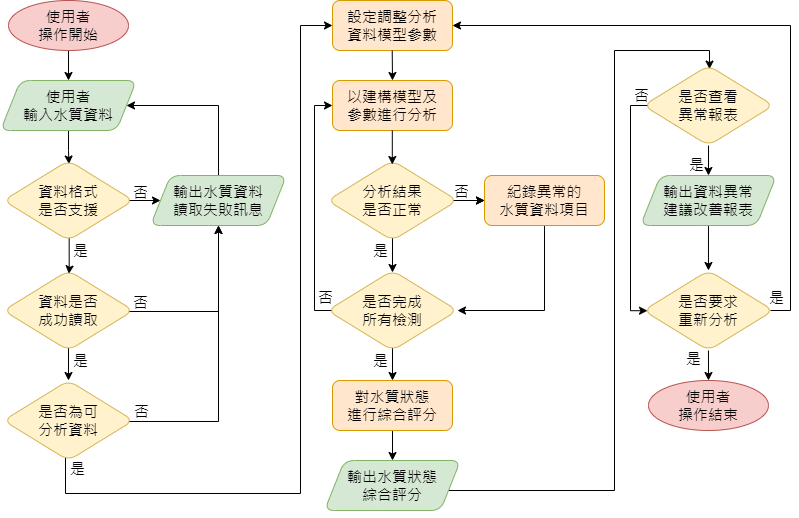
\includegraphics[width=0.6\textwidth]{resources/image/使用者流程圖.png}
        \caption{使用者流程圖}
        \label{fig:user_flow}
    \end{figure}
\item 執行進度\\
  本研究自2024年7月1日起開始執行,以甘特圖(Gantt Chart)進行嚴謹的規劃和執行,於2025年2月28日結案,共計執行約8個月。在8個月內完成了實作目標與相關內容,包括水質資料分析模型的比較、選擇與建構,以及智慧化水質分析與評估系統的開發與部署。研究主軸為找出最適合進行水質資料分析的模型並實際應用。各項步驟方向確認至最終完成如下表所示。
\item 遭遇之困難與解決途徑\\
  [內容 TODO]
\end{enumerate}

\item[(三)] 完成之工作項目及成果。
\begin{enumerate}[label=\arabic*.]
\item 完成之工作項目\\
  本研究執行期間完成之工作項目包括文獻回顧與探討、AI水質分析機器學習模型的訓練、進行實驗以比較不同機器學習模型對水質分析的效能差異、雲端伺服器架設與部署及智慧化水質分析與評估系統APP開發......等。
\item 完成之研究成果\\
  本研究計畫完成之研究成果大致可分為(3-2-1)AI水質分析機器學習模型比較及(3-2-2)智慧化水質分析與評估系統兩部分。兩部分詳細說明如下:
    \begin{enumerate}[label=3-2-\arabic*.]
        \item AI水質分析機器學習模型比較\\
          為能有效進行水質資料的分析與評估,研究重點為設計一個能達成計畫目標之機器學習模型。模型選擇如「(二)研究步驟」中「(2-2-3)模型選擇與比較」之內容所述。評估以線性迴歸(LR)、支援向量機(SVM)、隨機森林樹(RF)、多元多項式迴歸(MPR)、XGBoost及LightGBM進行比較,並選擇最適合進行水質資料分析的模型。最終成果將以模型的決定係數(R²)、均方根誤差(RMSE)及平均絕對誤差(MAE)等指標進行評估,並選擇最適合進行水質資料分析的模型。\\
          模型開發亦如「(二)研究步驟」之內容所述,以前期「運用智慧型綠能永續景觀噴泉促進環境保育效益之研究」計畫所蒐集之水質資料結合中華民國環境部全國環境水質監測資訊網的公開資料,共計87,005筆水質資料進行運用。並將開發之機器學習模型將部署於雲端平臺,提供大量水質資料處理所需的運算能力。\\
          為能有效評估水質資料,本研究使用水體品質指標(Water Quality Index, WQI$_5$)WQI能夠將大量水質資料轉換如等級一樣的數值,比起各種參數的一長算數值更容易理解與運用,使人們更容易理解水質資料呈現的結果\cite{ref35}。WQI的公式如公式(6)所示,同時,本研究在訓練過程中依照WQI$_5$版本為各項水質資料項目加上權重如表2所示,再依分析結果依表3進行評級,使分析結果具有客觀的可信度。\\
        \begin{equation}
            WQI_5 = \frac{\sum_{i=1}^5 (W_i Q_i)^{1.5}}{10}
        \end{equation}
            \begin{table}[H]
                \centering
                    \begin{minipage}[t]{0.45\textwidth}
                        \centering
                        \caption{WQI$_5$水質參數項目與權重}
                            \begin{tabular}{cc}
                            \hline
                            WQI$_5$ 水質參數項目 & 權重 \\
                            \hline
                            溶氧(DO) & 0.31 \\
                            生化需氧量(BOD5) & 0.26 \\
                            氨氮(NH3-N) & 0.19 \\
                            懸浮固體(SS) & 0.17 \\
                            電導率(EC) & 0.07 \\
                            \hline
                        \end{tabular}
                        \label{table:wqi_weights}
                    \end{minipage}
                    \begin{minipage}[t]{0.45\textwidth}
                        \centering
                        \caption{WQI$_5$水質指數範圍與評級}
                        \begin{tabular}{cc}
                        \hline
                        指數範圍 & 評級 \\
                        \hline
                        WQI$_5>100$ & N/A \\
                        $85<$WQI$_5\leq100$ & 優良 \\
                        $70<$WQI$_5\leq85$ & 良好 \\
                        $50<$WQI$_5\leq70$ & 中等 \\
                        $30<$WQI$_5\leq50$ & 不良 \\
                        $15<$WQI$_5\leq30$ & 糟糕 \\
                        $0<$WQI$_5\leq15$ & 惡劣 \\
                        \hline
                    \end{tabular}
                    \label{table:wqi_grades}
                    \end{minipage}
            \end{table}
            \begin{enumerate}[label=\Alph*.]
                \item AI水質分析機器學習模型殘差\\
                  
                \item AI水質分析機器學習模型指標\\
                  
            \end{enumerate}
        \item 智慧化水質分析與評估系統\\
    \end{enumerate}
\item 學術研究、國家發展及其他應用方面預期之貢獻\\
  本計畫旨在提供一個快速且準確,基於機器學習的智慧化水質評估方案,期望開發成果能成為解決水質問題的實用工具。本計畫在研究上需要結合跨領域的專業知識與技術,因此相關成果將在整理分析後進行論文發表,預計能對資訊工程、人工智慧、水資源管理和環境生態保育等領域產生有意義的價值與貢獻。
    \begin{enumerate}[label=3-3-\arabic*.]
        \item 參加 PyCon Taiwan 2024 臺灣 Python 年會 Poster Session
        \item 參加 2024 國際民生電子研討會並獲得論文佳作獎
        \item 前期計畫相關研究成果發表期刊並接受
    \end{enumerate}
\end{enumerate}

\begin{thebibliography}{99}
\bibitem{ref1} Shao, Z., Zhao, R., Yuan, S., Ding, M., \& Wang, Y. (2022). Tracing the evolution of AI in the past decade and forecasting the emerging trends. Expert Systems with Applications, 209, 118221.
\bibitem{ref2} Cowls, J. (2021). ‘AI for Social Good’: Whose Good and Who’s Good? Introduction to the Special Issue on Artificial Intelligence for Social Good. Philosophy \& Technology, 34(Suppl 1), 1–5. 
\bibitem{ref3} Aggarwal, K., Mijwil, M. M., Al-Mistarehi, A. H., Alomari, S., Gök, M., Alaabdin, A. M. Z., \& Abdulrhman, S. H. (2022). Has the future started? The current growth of artificial intelligence, machine learning, and deep learning. Iraqi Journal for Computer Science and Mathematics, 3(1), 115-123.
\bibitem{ref4} Zhou, Y., Wang, X., Li, W., Zhou, S., \& Jiang, L. (2023). Water Quality Evaluation and Pollution Source Apportionment of Surface Water in a Major City in Southeast China Using Multi-Statistical Analyses and Machine Learning Models. International Journal of Environmental Research and Public Health, 20(1). 
\bibitem{ref5} Im, Y., Song, G., Lee, J., \& Cho, M. (2022). Deep Learning Methods for Predicting Tap-Water Quality Time Series in South Korea. Water (20734441), 14(22), 3766. 
\bibitem{ref6} Imran, H., Al-Abdaly, N. M., Shamsa, M. H., Shatnawi, A., Ibrahim, M., \& Ostrowski, K. A. (2022). Development of prediction model to predict the compressive strength of eco-friendly concrete using multivariate polynomial regression combined with stepwise method. Materials, 15(1), 317.
\bibitem{ref7} Narayan, V., \& Daniel, A. K. (2022). Energy Efficient Protocol for Lifetime Prediction of Wireless Sensor Network using Multivariate Polynomial Regression Model.
\bibitem{ref8} Zeini, H. A., Lwti, N. K., Imran, H., Henedy, S. N., Bernardo, L. F. A., \& Al-Khafaji, Z. (2023). Prediction of the Bearing Capacity of Composite Grounds Made of Geogrid-Reinforced Sand over Encased Stone Columns Floating in Soft Soil Using a White-Box Machine Learning Model. Applied Sciences, 13(8), 5131.
\bibitem{ref9} Chen, T., \& Guestrin, C. (2016, August). XGBoost: A scalable tree boosting system. In Proceedings of the 22nd ACM SIGKDD International Conference on Knowledge Discovery and Data Mining (pp. 785-794). New York, NY, United States.
\bibitem{ref10} Ke, G., Meng, Q., Finley, T., Wang, T., Chen, W., Ma, W., ... \& Liu, T. Y. (2017). LightGBM: A highly efficient gradient boosting decision tree. Advances in Neural Information Processing Systems, 30.
\bibitem{ref12} McKinney W. (2022). Python for Data Analysis: Vol. Third edition. O’Reilly Media.
\bibitem{ref13} Harnowo, A. (2022). Blending a MOOC course into a Business School’s Course to Introduce Python for Data Analytics. Business Education Innovation Journal, 14(2), 31–35.
\bibitem{ref14} Harris, C. R., Millman, K. J., Van Der Walt, S. J., Gommers, R., Virtanen, P., Cournapeau, D., ... \& Oliphant, T. E. (2020). Array programming with NumPy. Nature, 585(7825), 357-362.
\bibitem{ref15} Nishino, R. O. Y. U. D., \& Loomis, S. H. C. (2017). Cupy: A numpy-compatible library for nvidia gpu calculations. 31st confernce on neural information processing systems, 151(7).
\bibitem{ref16} McKinney, W. (2012). Python for data analysis: Data wrangling with Pandas, NumPy, and IPython. " O'Reilly Media, Inc.".
\bibitem{ref17} Chen, D. Y. (2017). Pandas for everyone: Python data analysis. Addison-Wesley Professional.
\bibitem{ref18} Aurélien Géron. (2022). Hands-On Machine Learning with Scikit-Learn, Keras, and TensorFlow, 3rd Edition. O’Reilly Media, Inc.
\bibitem{ref19} Pedregosa, F., Varoquaux, G., Gramfort, A., Michel, V., Thirion, B., Grisel, O., ... \& Duchesnay, E. (2011). Scikit-learn: Machine Learn-ing in Python, Journal of Machine Learning Re-search, 12.
\bibitem{ref20} Hunt, J. (2023). Introduction to Matplotlib. In Advanced Guide to Python 3 Programming, Cham: Springer International Publishing, 121-128.
\bibitem{ref21} Bill Lubanovic. (2024). FastAPI. O’Reilly Media.
\bibitem{ref22} Bansal, P., \& Ouda, A. (2022, July). Study on integration of fastapi and machine learning for continuous authentication of behavioral biometrics. In 2022 International Symposium on Networks, Computers and Communications (ISNCC) (pp. 1-6). IEEE.
\bibitem{ref23} Native, R. (2020). React native. línea]. Disponible en: https://reactnative. dev/.[Último acceso: 2 de noviembre 2019].
\bibitem{ref24} Kotsiantis, S. B., Kanellopoulos, D., \& Pintelas, P. E. (2006). Data preprocessing for supervised leaning. International journal of computer science, 1(2), 111-117.
\bibitem{ref25} Burlig, F., Knittel, C., Rapson, D., Reguant, M., \& Wolfram, C. (2020). Machine learning from schools about energy efficiency. Journal of the Association of Environmental and Resource Economists, 7(6), 1181-1217.
\bibitem{ref26} Sharma, P., \& Singh, J. (2018, September). Machine learning based effort estimation using standardization. In 2018 International Conference on Computing, Power and Communication Technologies (GUCON) (pp. 716-720).  Greater Noida, NCR New Delhi, India.
\bibitem{ref27} Ajona, M., Vasanthi, P., \& Vijayan, D. S. (2022). Application of multiple linear and polynomial regression in the sustainable biodegradation process of crude oil. Sustainable Energy Technologies and Assessments, 54, 102797.
\bibitem{ref28} Verdonck, T., Baesens, B., Óskarsdóttir, M., \& vanden Broucke, S. (2024). Special issue on feature engineering editorial. Machine Learning, 113(7), 3917-3928.
\bibitem{ref29} James, G., Witten, D., Hastie, T., Tibshirani, R., \& Taylor, J. (2023). Linear regression. In An introduction to statistical learning: With applications in python (pp. 69-134). Cham: Springer international publishing.
\bibitem{ref30} Vapnik, V. (2013). The nature of statistical learning theory. Springer science \& business media.
\bibitem{ref31} Roy, A., \& Chakraborty, S. (2023). Support vector machine in structural reliability analysis: A review. Reliability Engineering \& System Safety, 233, 109126.
\bibitem{ref32} Breiman, L. (2001). Random forests. Machine learning, 45, 5-32.
\bibitem{ref33} Sinha, P. (2013). Multivariate polynomial regression in data mining: methodology, problems and solutions. Int. J. Sci. Eng. Res, 4(12), 962-965.
\bibitem{ref34} Berrar, D. (2019) Cross-Validation. In: Ranganathan, S., Gribskov, M., Nakai, K. and Christian Schönbach, C., Eds., Reference Module in Life Sciences Encyclopedia of Bioinformatics and Computational Biology, Vol. 1, Elsevier, Amsterdam, 542-545.
\bibitem{ref35} Abdul Hameed M Jawad, A., Bahram K, M., \& Abass J, K. (2010). Evaluating raw and treated water quality of Tigris River within Baghdad by index analysis. journal of water resource and protection, 2010.

\end{thebibliography}

\end{enumerate}	

\label{LastPage}
\end{document}